\documentclass{article}
\title{CUDA Parallel Programming\\Homework 7}
\usepackage{graphicx}
\usepackage[UTF8]{ctex}
\usepackage{hyperref}
 \hypersetup{
	colorlinks=true,
	linkcolor=blue,
	filecolor=blue,
	citecolor = black,      
	urlcolor=blue,
}
\usepackage{amsmath}
\usepackage[linesnumbered,ruled]{algorithm2e}
\CTEXoptions[today=old]
\author{40647007S 朱健愷}

\begin{document}
	\maketitle
	\section{Cloth Particle System Simulation}
	\subsection{Proposal}
	Particle system is the system that manages the particles' behavior. It accepts various forces as input and applies them into each particle, makes the particles in particle system move according to force applied on it.
	
	Particle system is often used to model some physical phenomenom, like spring, fluid, rigid body, cloth, etc. By applying different force and constraint, we can simulate their behavior by simulate them in every time step.
	
	Because nearly half of the particle's behavior can be computed independently, so it's suitable for using CUDA to compute them. The other portion of it needs some particle to cooperate with the other to achieve the computation, they can be handled using CUDA but probably need more work on them.
	
	To construct the particle system, we have following component used in particle system.
	\begin{itemize}
		\item Particle - Basic element in particle system, each particle store their position, velocity, force and mass. We can add other quantity according to our demand.
		\item Solver - A numerical method to solve each particle's behavior in each time step, because the methematic from applying force to control the particle's position according to applied force involves integration, so we need a numerical solver to compute the integration result numerically.
		\item Force - A factor to drive the particle's movement, e.g. gravity force offers a constant acceleration for each particle's velocity to fall down, damp force "prevents" the particle's velocity from getting larger, spring force "drags" the particle who leaved their rest position.
		\item Constraint - A factor to constraint the particle's movement, e.g. pin constraint prevents particles from getting away their position, collision constraint prevents particles from colliding to other particle or wall, etc.
	\end{itemize}
	\subsection{Motivation}
	One of my courses is about making special CG effect myself, in that course I'm forced to implement a complex particle system all by myself, including look up various material, implement the algorithm, etc. One thing that keep annoying me is that when doing long time step, complex simulation on large particle system simulation, the calculation executed in CPU only environment always demands numerous time. So I thought that if a proportion of calculation is independent, why don't I calculate them simply from GPU? Furthermore, I can use my knowledge learned in this course to accelerate the calculation, it may be a good practice to implement them.
	
	\subsection{Kind of force in cloth simulation}
	\subsubsection{Spring Force}
	The spring force has two form, one is for per particle, two is for a spring modeled by 2 particles.
	
	The first form is $F=-kx$, where $F$ is the spring force vector, $k$ is the stiffness constant, $x$ is the rest location. This force trys to make particle stay in their rest location.

	The second form is $F=k(L_0-\left\lVert p-q\right\rVert)$, where $F$ is the spring force vector, $k$ is the stiffness constant, $L_0$ is rest length, $p$ and $q$ are the position of two particles. This force trys to make two particles stay close to their rest length.

	\subsubsection{Gravity Force}
	The gravity force makes the particle to fall down, its form is 
	\begin{equation}
		F=\left [0, -mg, 0\right ]^T
	\end{equation}
	where $m$ is the particle's mass, $g$ is the gravity constant, usually set to 9.8.
	
	\subsubsection{Damping Force}
	The damping force trys to make the particle's velocity drop, its form is $F=-cv$, where $F$ is the damping force vector, $c$ is the damping constant, $v$ is the particle's velocity.
	\subsection{Kind of constraint in cloth simulation}
	\subsubsection{Pin Constraint}
	The pin constraint force particle to stay in their position no matter what force applied on it. It is done by make the particle's velocity vector to zero vector to prevent it from moving.
	
	\subsubsection{Collision Constraint}
	The collision constraint prevent cloth modeled by particles from interpenetrating to each other, this is the most complex part of cloth simulation, since it involved in  checking of multiple particle pairs if they haved collision and solving their collision by apply some repulsion force.
	\section{Algorithm}
\begin{algorithm}
	\SetKwInOut{Input}{Input}
	\SetKwInOut{Output}{Output}
	
	\underline{function ParticleSystemSimulation} $(p, v, m)$\;
	\Input{End time step $T$\\Each time step $dt$\\Each particle's initial position $p$, velocity $v$, mass $m$}
	\Output{Each particle's position, velocity in each time step}
	$t\gets 0$\;
	\For{$t \le T$}
	{
		Calculate various forces into each particle's acceleration using Newton's second law\;
		Apply acceleration into each particle velocity\;
		Apply various constraints to each particle\;
		Update each particle's position and velocity using solver\;
		$t  += dt$\;
	}
	\caption{Overall particle system simulation framework}
\end{algorithm}
	\subsection{Implementation with CUDA}
	All of the code in "for loop" of this algorithm can be done by CUDA, eg. apply spring force involves calculate $f=-kx$. I can simply distribute the computation into each thread and block to calculate every particles' acceleration according to Newton's secod law $a=\frac{f}{m}$, where $f$ is the force applied on the particle, $m$ is the mass of the particle, $a$ is the corresponding particle's acceleration, this accumulated particle acceleration can later be applied on particle's velocity using CUDA. 
	
	Finally, constraint like collision constraint are used to check out whether particles collided to other, this might be done through several iteration, each iteration group particles which are already collided with others into blocks according to their spatial relation, and solve their collision in block(I need to read more material and experiment it to verify my thoughts).
	\section{Expected result}
	I expected to use the particle system simulation to simulate the cloth behavior like the figure shown below.
	\begin{figure}
		\centering
		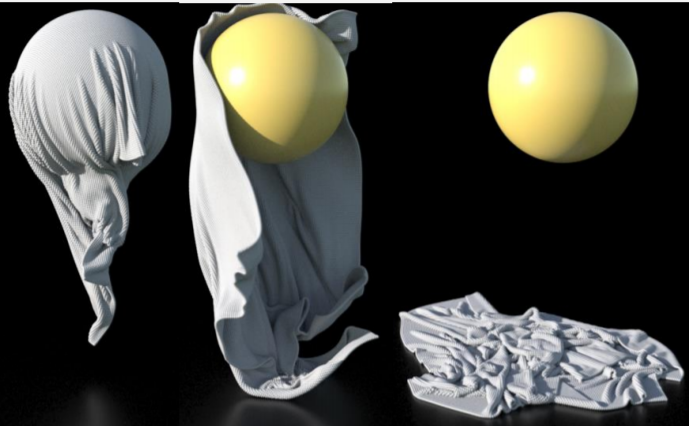
\includegraphics[width=0.6\linewidth]{ref1}
	\end{figure}
	\section{Current result}
	I've implemented some code executed in CPU, one figure shown below are the current result, using only pin constraint on top 2 particles, small spring force to maintain the cloth structure, 2nd order Runge-Kutta solver method to calculate the force applied on it.
	\begin{figure}[hb!]
	\centering
	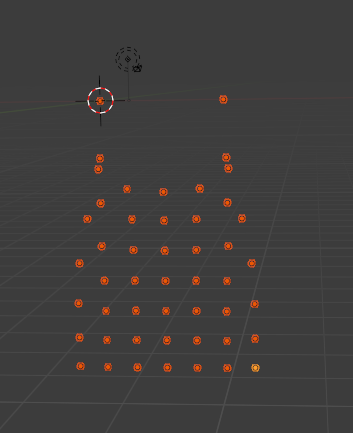
\includegraphics[width=0.45\linewidth]{ref2}
	\end{figure}
	\section{Reference}
	\href{https://hackmd.io/HqFfw6ydSMe1-X-guUFJSA}{My own particle system simulation note(In it include each reference I searched)}
	
	\href{https://www.ics.uci.edu/~shz/courses/cs114/docs/proj3/index.html}{Cloth simulation assignment}
\end{document}